
%(BEGIN_QUESTION)
% Copyright 2006, Tony R. Kuphaldt, released under the Creative Commons Attribution License (v 1.0)
% This means you may do almost anything with this work of mine, so long as you give me proper credit

The following pneumatic transducer converts between a 3-15 PSI signal range and a 6-30 PSI signal range.  Based on the illustration shown here, which pressure range corresponds to the input and which pressure range corresponds to the output?  Does it input 3-15 PSI and output 6-30 PSI, or vice-versa?  How can you tell??

$$\includegraphics[width=15.5cm]{i00203x01.eps}$$

\underbar{file i00203}
%(END_QUESTION)





%(BEGIN_ANSWER)

The input pressure range is the lesser of the two (3-15 PSI), and the output is the greater of the two (6-30 PSI).

\vskip 10pt

Follow-up question: explain how the following op-amp circuit is similar to the pneumatic system shown in the question.

$$\includegraphics[width=15.5cm]{i00203x02.eps}$$

%(END_ANSWER)





%(BEGIN_NOTES)


%INDEX% Relay, converter: pneumatic pressure-to-pressure

%(END_NOTES)


